\begin{figure}[htp]

\begin{subfigure}{\textwidth}
\begin{subfigure}{0.45\textwidth}
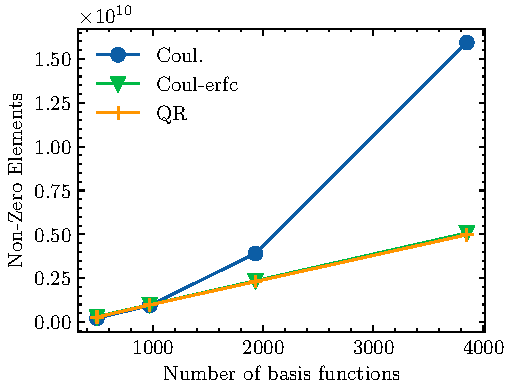
\includegraphics[width=\textwidth]{../articles/art1/ftmp2_nze_alkan}
\end{subfigure}
\hfill
\begin{subtable}{0.45\textwidth}
\begin{tabular}{rrrr}
\hline
N$_{AO}$ & DFCM & DFCAM & QRDF \\ \hline
490 & --- & --- 	& --- \\ 
970	& 2.14 & 1.69 & 1.80 \\
1930	 & 2.06 & 1.26 & 1.25 \\
3850	 & 2.03 & 1.11 & 1.11 \\
 \hline
\end{tabular}
%\captionof{table}[This Table]{REDO THIS!!!!}
\end{subtable}
\caption{}
\label{fig:GS_ZMEM_LA}
\end{subfigure}

\vspace{1.5\baselineskip}

\begin{subfigure}{\textwidth}
\begin{subfigure}{0.45\textwidth}
\centering
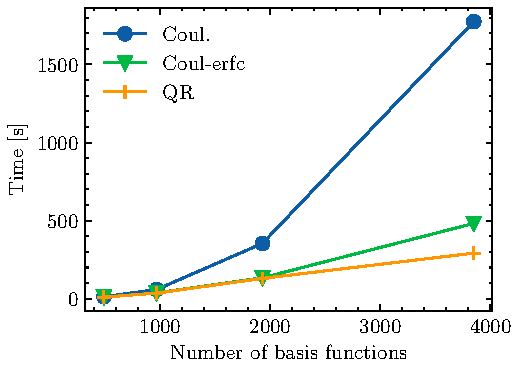
\includegraphics[width=\textwidth]{../articles/art1/mp2_alkan}
%\captionof{figure}[This Figure]{Figure}
\end{subfigure}
\hfill
\begin{subtable}{0.45\textwidth}
\centering
\begin{tabular}{rrrr}
\hline
N$_{AO}$ & DFCM & DFCAM & QRDF \\ \hline
490 & --- & --- 	& --- \\ 
970	& 2.45 & 1.96 & 2.09 \\
1930	 & 2.55 & 1.82 & 1.83 \\
3850	 & 2.00 & 1.59 & 1.00 \\
 \hline
\end{tabular}
%\captionof{table}[This Table]{REDO THIS!!!!}
\end{subtable}
\caption{}
\label{fig:GS_ZSCALE_LA}
\end{subfigure}

\vspace{1.5\baselineskip}

\begin{subfigure}{\textwidth}
\begin{subfigure}{0.45\textwidth}
\centering
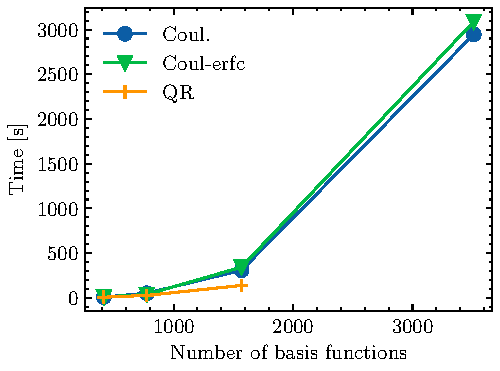
\includegraphics[width=\textwidth]{../articles/art1/mp2_fw}
%\captionof{figure}[This Figure]{Figure}
\end{subfigure}
\hfill
\begin{subtable}{0.4\textwidth}
\centering
\begin{tabular}{rrrr}
\hline
N$_{AO}$ & DFCM & DFCAM & QRDF \\
\hline 
490 & --- & --- & --- \\ 
970 & 2.51 & 1.88 & 1.88 \\ 
1930 & 2.59 & 3.18 & 2.36 \\ 
3850 & 3.26 & 3.18 & --- \\ 
 \hline
\end{tabular}
%\captionof{table}[This Table]{REDO THIS!!!!}
\end{subtable}
\caption{}
\label{fig:GS_ZSCALE_FW}
\end{subfigure}

\caption{(a) Sparsity behavior of the intermediate tensor $\mbf{D}$ in the Z kernel for the first Laplace point. (b) Average wall times for the construction of the Z kernel and scaling coefficients (LA). (c) Average wall times for the construction of the Z kernel and scaling coefficients (FW).}

\end{figure}